\title[EG \LaTeX\ Author Guidelines]%
      {Volumetric Ray Tracing}

% for anonymous conference submission please enter your SUBMISSION ID
% instead of the author's name (and leave the affiliation blank) !!
\author[1062]
%{\parbox{\textwidth}{\centering D.\,W. Fellner\thanks{Chairman Eurographics Publications Board}$^{1,2}$
 %      and S. Behnke$^{2}$
 {\parbox{\textwidth}{\centering 1062$^{1}$
%        S. Spencer$^2$\thanks{Chairman Siggraph Publications Board}
        }
        \\
% For Computer Graphics Forum: Please use the abbreviation of your first name.
{\parbox{\textwidth}{\centering $^1$OTH Regensburg, Germany
%        $^2$ Another Department to illustrate the use in papers from authors
%             with different affiliations
       }
}
}
% ------------------------------------------------------------------------

% if the Editors-in-Chief have given you the data, you may uncomment
% the following five lines and insert it here
%
\volume{2021}   % the volume in which the issue will be published;
\issue{1}     % the issue number of the publication
% \pStartPage{1}      % set starting page


%-------------------------------------------------------------------------
\begin{document}


\maketitle
%-------------------------------------------------------------------------
\begin{abstract}

\end{abstract}  
%-------------------------------------------------------------------------
---START OF REVIEW---
\section{Introduction}
In Computer Graphics, objects usually are represented as a set of geometric primitives (e.g. triangles), displaying the surface of the object in question. However, this approach is not always suitable. For example, if the original data representation of the object is volumetric data (which might be produced by medical 3d scans\cite{511}), the traditional rendering technique would necessitate the creation of an intermediate surface representation that might introduce unwanted artifacts. Another issue arises if the object has no well-defined surfaces to which geometric primitives could be fitted, such as a cloud or fog\cite{10.1145/964965.808594}. In such cases, volumetric ray tracing might be used, a technique in which rays are cast through a volume which contains information about its optical properties(e.g color and opacity), sampled at various points within the volume, accumulated and projected on a 2d image (see figure 1)\cite{511}. A description of this algorithm is presented in this paper, alongside several strategies for improving computational speed, such as (probabilistic) early termination of a ray, and sampling at lower resolutions within the volume.

\section{Mathematical Theory Behind Volumetric Ray Tracing}
Volumetric ray tracing follows the same basic principle as classical ray tracing in which an image is rendered by spanning a pixel plane in front of the camera and casting one or multiple rays through each pixel.
That means for a point $\vec{x}$ on the plane we cast a ray in direction $-\omega$ and calculate the amount of light $\vec{x}$ receives from direction $\omega$, called $L(\vec{x},\omega )$.
To do this, we calculate $\vec{y}$, the closest intersection point of the ray with a piece of geometry. At $\vec{y}$, we calculate the amount of light transported from $\vec{y}$ in direction $\omega$ (either through reflection or emission), called $L_e(\vec{y},\omega )$ (The exact method for calculating $L_e$ is a topic of classical raytracing and will not be further evaluated in this paper. In the following, we assume $L_e$ to be a known quantity).
Thus, we get the equation 
\begin{equation}
L(\vec{x},\omega ) = L_e(\vec{y}, \omega )
\end{equation}
However, this equation assumes that the light has no interactions between $\vec{x}$ and $\vec{y}$, which is only true if the ray travels through a vacuum. If the light travels through a medium that interacts with if (called a participating medium), the interactions change the light along the ray. In most cases, these interactions are small enough to be ignored, but in certain scenarios (e.g if there is fog, clouds or smoke present) they might have a noticeable effect. The types of interactions we need to consider are absorption, emission, in-scattering and out-scattering.

Absorption and out-scattering attenuate the light intensity along the ray, in-scattering and emission add to it.
\subsection{Absorbtion And Out-Scattering}
Firstly, let us consider only out-scattering and absorption, which occur due to tiny particles floating around in the volume (such as water droplets in clouds and fog, or dust particles in the air).
Of course, these particles are far too numerous to be directly simulated, but their distribution in 3D space can be stochastically modeled (similar to how detailed surface structures can be modeled by micorfacets in classical ray tracing).

To do so, consider a close-up look at a ray section traveling through the vloume [CITATION!].
This section can be assumed to be a cylinder with a base area $E$ and a height $\DELTA h$, through which the ray travels from top to bottom.
Within this cylinder, there exists a certain number of out-scattering and absorbing particles, defined as $n_s={\ro}_sE{\DELTA}h$ and $n_a={\ro}_aE{\DELTA}h$ respectively, where ${\ro}_s$ and ${\ro}_a$ are the densities of the particles.
From the top-down view, the particles will occupy an area of $n_sA={\rho}_sAE{\DELTA}h \over E$ and f $n_aA={\rho}_aAE{\DELTA}h \over E$, respectively, if we assume that the particles do not overlap each other, which is reasonable if the densities and the height do not become too large.
This can be simplified to ${\rho}_sA{\DELTA}h$ and ${\rho}_sA{\DELTA}h$, which gives us the fractions of light which are stopped in the cylinder, either through absorbtion or out-scattering. By letting $\DELTA h$ approach 0, we see that for each infinitessimaly small cylinder slice with height $dh$, the change in intensity is proportionally to $-({\rho}_sA + {\rho}_aA)dh$.
Formulated as a differential equation, this results in
\begin{equation}
dL = -(-({\rho}(h)_sA + {\rho}(h)_aA)L(h)dh
\end{equation}
At this point, we introduce the scattering coefficient ${\mu}_s ={\rho}(h)_sA $, the absorption coefficient ${\mu}_a = {\rho}(h)_aA$ and the extinction coeffcient ${\mu}_t = {\mu}_s +{\mu}_a$, which give a measure of how much light is lost due to scattering, to absorption, and in total. Thus, equation [REFERNCE] can be simplified to
\begin{equation}
dL = - {\mu}_t(h)L(h)dh
\end{equation}
which solution is
\begin{equation}
L(h) = L_0e^{-\int_{0}^{h} {\mu}_t(s)ds}
\end{equation}
Rearranging this equation gives
\begin{equation}
L(h) \over  L_0 = e^{-\int_{0]^{h} {\mu}_t(s)ds}
\end{equation}
meaning, that the calculated integral $e^{-\int_{0]^{h} {\mu}_t(s)ds}$ gives us the ratio of the light that travels through a cylinder of height $h$ unimpeded. In the following, we call this quantity the transmittance, and refer to it as $\tau(\vec{x), \vec{x'})$ (the ratio of light that arrives at $\vec{x}$ from $\vec{x'}$).
Thus, going back to equation [REFERENCE], we can now specify how much $L_e$ gets attenuated, and get the equation
\begin{equation}
L(\vec{x},\omega ) =\tau(\vec{x), \vec{y}) L_e(\vec{y}, \omega )
\end{equation}
However, this is not correct either, since we still need to consider in-scattering and emission along the ray.
\subsection{Emission And In-Scattering}
For this purpose, let us consider any arbitrary point $\vec{u}$ on the ray from $\vec{x}$ to $\vec{y}).
At $\vec{u}$, the particles of the medium emit some light towards $\omega$, which we call $\epsilon (\vec{u}, \omega )$. In our cylindrical model, the amount of absorbing particles at position $\vec{u}$ is ${\mu}_a(\vec{u})$. We assume that the particles responsible for absorbtion are also responsible for emission, meaning the amount of light emitted at $\vec{u}$ towards $\omega$ is ${\mu}_a(\vec{u})\epsilon (\vec{u}, \omega )$.
In-scattered light can arrive at $\vec{u}$ from every direction, which means we need to integrate over the sphere:
\begin{equation}
\int_{\OMEGA} L(\vec{u}, \omega `)d\omega `
\end{equation}
However, not all light arriving at $\vec{u}$ is scattered towards $\omega $. The so called phase function $f_p(\vec{u}, \omega , \omega `)$ gives us the ratio light arriving at $\vec{u}$ from $\omega `$ being reflected towards $\omega$. In this sence, the phase function in analogous to the BDRF in classical ray tracing. Furthermore, the amount of light scattered towrds $\omega $ also depends on the number of in-scattering particles present at $\vec{u}$. We assume that in-scattering particles are equal to out-scattering particles and get the equation
\begin{equation}
L_e^s(\vec{u}, \omega ) = {\mu}_s(\vec{u})\int_{\OMEGA} f_p(\vec{u}, \omega , \omega `)L(\vec{u}, \omega `)d\omega `  + {\mu}_a(\vec{u})\epsilon (\vec{u}, \omega )
\end{equation}
describing the total amount of light being added to the ray at $\vec{u}$. We call this quantity $L_e^s$ and use the superscript $s$ to differentiate it from $L_e$.
However, not all of $L_e^s(\vec{u}, \omega )$ arrives at $\vec{x}$, since the newly added light also needs to travel through the volume where it is attenuated by the transmittance $\tau (\vec{x}, \vec{u})$.
To get the total amount of light added to the ray, we sum up the light contribution of all points along the ray by integrating over the ray:
\begin{equation}
\int_{\vec{x}}^{\vec{y} \tau(\vec{x}, \vec{u})L_e^s(\vec{u}, \omega )d\vec{u}
\end{equation}
\subsection{The rendering Equation}
Adding this to the light arriving from $\vec{y}$ gives the total amount of light arriving at $\vec{x}$ from $\omega $.
\begin{equation}
L(\vec{x}, \omega ) = \int_{\vec{x}}^{\vec{y} \tau(\vec{x}, \vec{u})L_e^s(\vec{u}, \omega )d\vec{u} + \tau(\vec{x), \vec{y}) L_e(\vec{y}, \omega )
\end{equation}
This integral is complicated to solve, especially since the expressin $L(\vec{x}, \omega )$ appears on both sides of the equation.
In the following, we will discuss several methods for approximating a solution.




\section{Basic Volumetric Ray Tracing Algorithm}
In this chapter we will discuss an algorithmic solution to a simplified version of the rendering equation we derived in the previous section.
\subsection{Simplified Rendering Equation}
In the following, we will ignore all scattering effects in the medium and assume that the medium only absorbs and emitts light, which can be understood as a scenario where all external light has been completly evenly scattered within the volume. This is analogous to only rendering ambient lighting in classical ray tracing, whic assumes that the light is evenly distributed in the scene.
Furthermore, we will also ignore all other geometry in the scene and only focus on the volume. Thus, the term $\tau(\vec{x), \vec{y}) L_e(\vec{y}, \omega )$, which desribes the light contribution from the nearest intersection with a piece of geometry, is omitted.
Thus, we arrive at the equation
\begin{equation}
L(\vec{x}, \omega ) = \int_{\vec{x}}^{\vec{y} \tau(\vec{x}, \vec{u}){\mu}_a(\vec{u})\epsilon (\vec{u}, \omega)d\vec{u}
\end{equation}
For this chapter, we assume that the medium is contained within a cuboid boundary. Since there is no geometry, we can't cast the ray until it intersects with the geometry. Instead, the endpoint $\vec{y}$ of the ray will be the point where the ray leaves the cuboid boundary.

\subsection{Algorithmic Approximation To The Simplified Equation}
$L(\vec{x},\omega )$ is approximated by casting a ray in direction $-\omega$ and sampling it at evenly spaced points along the ray and summing up their contributions. The distance $d$ between the sampling points should be smaller than the volumes nyquist limit.
We start sampling at the first point within the volume, which has a distance of $d_0$ to $\vec{x}$. The $i$-th sample point then is described by
\begin{equation}
p_i=\vec{x} + d_0(-\omega) + di(-\omega)
\end{equation}
The light contribution of a point $p_i$ is considered to be the light contribution of the ray segment between $p_{i-1}$ and $p_i$.
\begin{equation}
\int_{p_{i-1}}^{p_i} \tau (p_0,p_{i-1}) \tau(p_{i-1},p_{i'} \mu_a(p_{i'})\epsilon (p_{i'}, \omega)dp_{i'}
\end{equation} 
As a necessary simplification, we assume all variables to be piecewise constant on the ray segments. This yields
\begin{equation}
\int_{p_{i-1}}^{p_i} \product_{1\le j \le i}(\tau(p_{j-1}, p_j)) \mu_a(p_{i})\epsilon (p_{i}, \omega)dp_{i}
\end{equation} 
\begin{figure}[htb]
  \centering
  % the following command controls the width of the embedded file
  % (relative to the width of the current column)
  %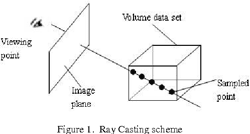
\includegraphics[width=.8\linewidth,natwidth=250,natheight=134]{RayCasting1.png}
  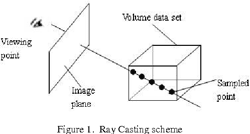
\includegraphics[width=.8\linewidth]{RayCasting1.png}
  \parbox[t]{.9\columnwidth}{\relax}~\cite{Appa2015RayCF}
  %
  \caption{\label{fig:firstExample}
          Illustration of the ray casting process.}
\end{figure}
\subsection{Terminology}
To enable a clear understanding in this section we will shortly define key terminology used in this paper. A voxel is an infinitesimally small point in 3D space with an associated vector value, that represents the color of that voxel. In this paper, these voxels are arranged in a regular cube lattice (although other arrangements are possible as well). A cell or area of influence of a voxel $v$ is defined as the region of space which is closer to $v$ than to any other voxel (meaning a cube in space with $v$ in the center). A voxel cube is defined as a group of 8 voxels that form a cube in space. The neighborhood of a voxel $v$ is defined as the set that includes $v$ as well as its 26 neighbors in 3D space. Since different authors use different notations, this terminology might be used slightly different in other papers.
\subsection{Underlying Volume Data}
In this paper, we consider the topic of synthesizing a 2d image from a 3d volume.
A volume can either be some continuous, ternary function (such as perlin or simplex noise\cite{10.1145/325165.325247}, which can be used to render volumetric clouds\cite{haggstrom2018real}), or a discrete 3d array\cite{511}.
Similar to a 2d image that consists of pixels that can be addressed by a 2d vector $\vec{x} \in \mathbb{N}^2$, a 3d array consists of voxels that are addressed by a 3d vector $\vec{x} \in \mathbb{N}^3$. [REFORMULATE?]The color of a voxel at position $\vec{x}$ is called $c(\vec{x})$, the opacity $\alpha(\vec{x})$ and the complete vector $v(\vec{x})$. The opacity is a scalar value, the color may also be a scalar value (for grayscale volumes) or a 3d vector (for colorful volumes).
To address the components of a vector $\vec{v}$, following notation is used:
\begin{equation}
	\vec{v}_{x}, x \in s{r, g, b, \alpha}
\end{equation}
 In the following, all values are assumed to be normalized to between 0 and 1. To project this volume to a image, for each pixel in the image a ray is cast through the volume and sampled at multiple, evenly spaced points on the ray (see figure 1)\cite{10.1145/78964.78965}.

\subsection{Volumetric Ray Tracing}
Like in the classical ray tracing algorithm, volumetric ray tracing works by casting a ray (or multiple rays if multisampling is used) for each pixel in the image that is to be created.

These rays are described by the equation $\vec{o} + t \cdot \vec{d}$, where $\vec{o}$ is the origin of the ray and $\vec{d}$ the direction. On each ray evenly spaced sample points are placed whose position is described by 
\begin{equation}
\vec{o} + n \cdot s \cdot \vec{d}
\end{equation}
for the n-th sample point. $s$ is a scale factor, determining how far apart the sample points are. $s$ should be roughly equal to the distance between voxels (this distance is assumed to be 1 in the volume model, but depending on the volumes world matrix this might be different in world coordinates), since a too great mismatch between sampling and voxel frequency woul lead to aliasing.
In the follwing, only sample points within the volume are considered. Those sample points then are sampled and composited together, resulting in a final color value for the image pixel.
\subsection{Interpolation}
The sample points on the ray are in general part of $\mathbb{R}^3$. This is no problem if the volume is described by a continuous function, which is defined everywhere. However, if it is a discrete 3d array only defined for points in $\mathbb{N}^3$, the value of the volume at the sample point must be interpolated.
 This interpolation is done over the 8 closest voxels to the sample point (usually with a trilinear interpolation). The opacity values can be interpolated regularly, but the color values must be weighted with the respective opacity values before interpolation \cite{729595}. To see why this is necessary, consider figure 2, which presents a simplified 2d example of a completely  opaque, white object behind completely transparent empty space. Naively interpolating in this volume would result in two sample points, one completely white and opaque, the other gray and semitransparent. This gray point is not present in the original data and is an unwanted artifact. Weighting the colors with their opacity prevents this from happening.
 \begin{figure}[htb]
  \centering
  % the following command controls the width of the embedded file
  % (relative to the width of the current column)
  %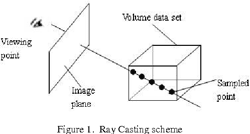
\includegraphics[width=.8\linewidth,natwidth=250,natheight=134]{RayCasting1.png}
  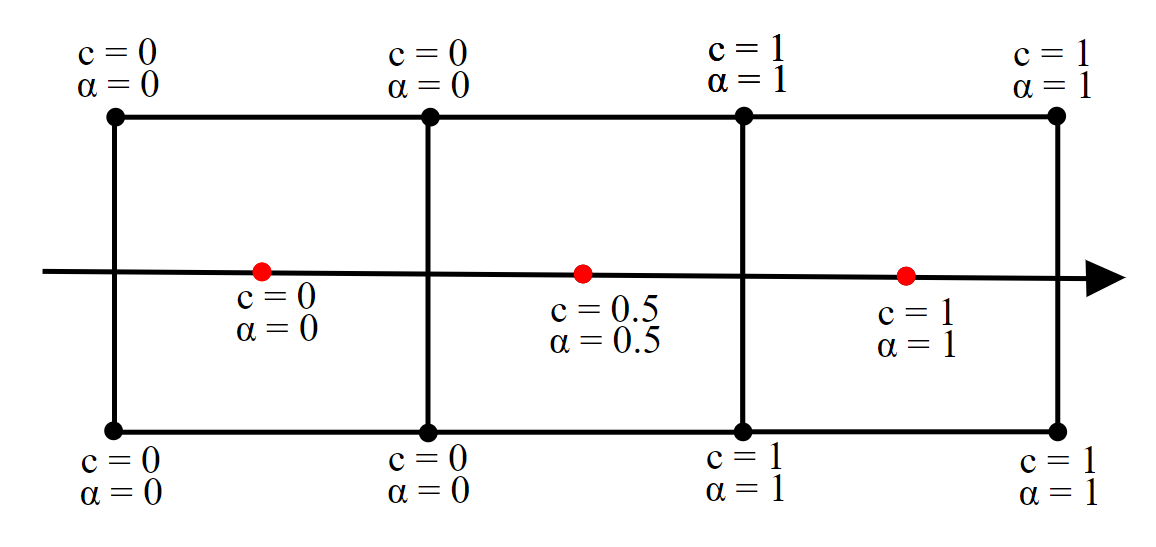
\includegraphics[width=.8\linewidth]{weighted_interpolation.png}
  \parbox[t]{.9\columnwidth}{\relax}
  %
  \caption{\label{fig:firstExample}
          Simplified visualization of naive interpolation in 2 dimensions. The black dots represent the voxels, the red dots the sample points. Notice that the second sample point has a gray color, even though the original data only has white voxels and blck, transparent voxels, which shouldn't affect the final color. Adapted from Wittenbrink et al.\cite{729595}}
\end{figure}
 \subsection{Compositing Of Multiple Sample Points}
To compose the various sampled points on the ray to a single pixel, the points one after the other are alpha blended together. This compositing can be done front to back\cite{Sabella1988ARA, Upson1988VbufferVV } (starting with the sample point closest to the camera, blending it with the second, then the third, and so on), or back to front\cite{10.1145/378456.378484, 511} (vice versa).  Usually, the back to front approach is chosen since it allows to optimize the computation\cite{10.1145/78964.78965} (see below).
 In the following, $c(i)$ is the color of the i-th sample point, and $\alpha(i)$ the opacity. The accumulated opacity 
 \begin{equation}
 \beta(i) = 1 - \prod_{j=1}^{i}(1 - \alpha(j))
 \end{equation}
 is the fraction of light absorbed between the first and i-th sample point. The final color $c_f$, which is displayed in the projected image, is then
 \begin{equation}
 c_f = \sum_{i=1}^n((1-\beta(i)) * c(i))
 \end{equation}
 if the ray has n sample points\cite{10.1145/147130.147155}.
\section{Optimization Strategies}
\subsection{Adaptive Termination Of Ray Tracing}
When looking at the compositing process described above, it becomes apparent that the contribution of a sample point to the final result decreases, the more other opaque sample points lie before it\cite{10.1145/78964.78965}. For an extreme example, consider figure 3. Here, all sample points behind the fully opaque black wall contribute nothing to the final value and can therefore be ignored. In other words, going back to equation (2), the ray casting can be terminated after the accumulated opacity reaches 1, without changing the image quality. If some errors in the image are acceptable, the threshold value for terminating the ray tracing might be chosen to be somewhat lower.
 \begin{figure}[htb]
  \centering
  % the following command controls the width of the embedded file
  % (relative to the width of the current column)
  %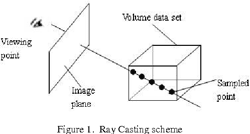
\includegraphics[width=.8\linewidth,natwidth=250,natheight=134]{RayCasting1.png}
  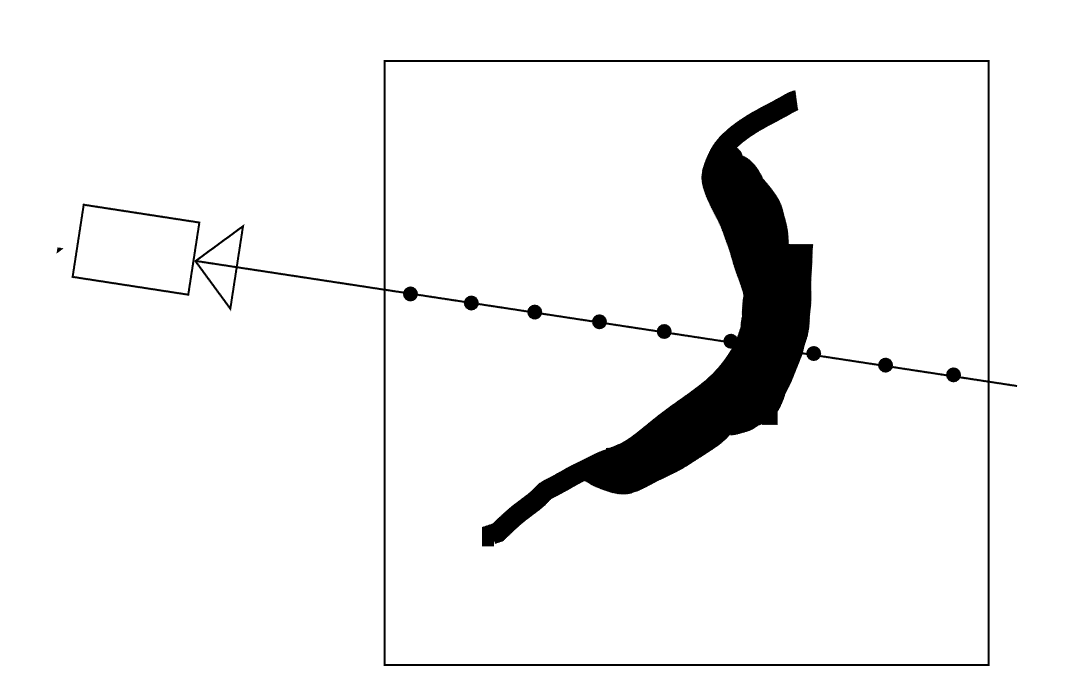
\includegraphics[width=.8\linewidth]{wall.png}
  \parbox[t]{.9\columnwidth}{\relax}
  %
  \caption{\label{fig:firstExample}
         The black, opaque object blocks parts of the volumes behind it. The samples behind the object (from the cameras perspective) are not visible and therefore irrelevant. }
\end{figure}
\subsection{Ray Termination With Russian Roulette}
The above described termination after a certain threshold is reached creates a bias in the synthesized image\cite{10.1145/97880.97886}. One way to avoid this is to use Russian Roulette to decide when to terminate a ray\cite{10.1145/147130.147155}. Unlike the above described approach, Russian Roulette terminates a ray only with a certain likelihood once the accumulated opacity reaches the threshold. The weight of the surviving rays is increased proportionally to compensate for the terminated rays.

\subsection{Pyramid Data Structures}
The follwing optimizations require a data structure called a pyramid. Pyramids are created from 3d arrays, if the volume to be rendered is defined as a function an intermediate array representation must be created.
Analogous to a mip-map which is a set of 2d arrays with decreasing resolution, a pyramid is a set of 3d arrays with decreasing resolution. The different volumes of which the pyramid consits are called the levels of the pyramid. The lowest level (called level 0) has the highest resolution, each succesive level has half the resolution than the preceeding one. To ensure that each level covers the same region in 3d space, the distance between the voxels are doubled each level.

--FIGURE!
In the follwing, we will make use several different kinds of pyramids, namely average, maximum and range pyramids.
\subsection{Average Pyramid}
The lowest level of the average pyramid is equal to the original 3d array, padded with zeros so that its size is a power of 2 in all dimensions.
The next level is created by aggregating the average of a cube of 8 voxels in the lower level to one voxel in the higher level. The voxel in the higher level is called the parent, the 8 lower voxels are called the children. This process is repeated until the last level, consisting of only one voxel, is reached. 
Similarily to the original volume, the pyramid can be sampled by interpolating the 8 closest voxels to the sample point. Consider however, that the primary purpose of the average pyramid is to enamble an approximation of the original data that is computationally faster than to render the original data.
The time complexity of rendering 3D data however does not depend on the number of voxels, but rather the number of samples along the ray (at first glance, this seems to imply that the average pyramid is superfluous and that the same could be accomplished by taking fewer sampling points in the original volume. This however would lead to a sample frequency significantly lower than the voxel frequency and thus to aliasing). If we therefore wish to cut the rendering time in half for each level we move up the pyramid, the amount of sampling points must be halfed and the distance between the sampling points must be doubled. This means that one sample in level $n+1$ should approximate two samples at level $n$. To achieve this, the sample at level $n+1$ must be blended with itself, since in level $n$ two samples are blended as well.


\subsection{Maximum And Minimum Pyramids}
A maximum pyramid works similar to an average pyramid, but the construction of level $0$ is somewhat different. A voxel in level $0$ at position $\vec{x}$ is created by taking the maximum of the $27$ voxels in the original dataset, that form a 3 by 3 cube around $\vec{x}$. Once the lowest level is created the succeding levels are constructed llike in the average pyramid, only that the maximum is used as the aggregation method, and not the maximum. Sampling a maximum pyramid is different from sampling an average pyramid. Since the maximum pyramid stores maxima, interpolating between different maxima would lead to wrong results. Instead, nearest neighbor interpolation is used (unlike in the average pyramid, the sample does not need to be blended with itself).
The minimum pyramid works analogously.
In the following, the sample taken at location $\vec{x}$ in the maximum pyramid at level $n$ is called $pyr_{max}(\vec{x}, n)$, and the sample in the minimum pyramid is called $pyr_{min}(\vec{x}, n)$.

\subsection{Range Pyramid}
The range pyramid is calculated by taking the difference between the maximum and minimum pyramid. Both the maximum and minimum pyramid store vectors (2D or 4D, depending on wether the underlying data is grayscale or colorful). To express the difference in a scalar, the diffrence of the components is summed up and normalized to the range of 0  and 1:
\begin{equation}
pyr_{range}(\vec{x}, n) = 1 \over 4 \cdot ((pyr_{max}(\vec{x}, n)_{r} - pyr_{min}(\vec{x}, n)_{r}) + (pyr_{max}(\vec{x}, n)_{g} - pyr_{min}(\vec{x}, n)_{g}) +(pyr_{max}(\vec{x}, n)_{b} - pyr_{min}(\vec{x}, n)_{b}) + (pyr_{max}(\vec{x}, n)_{\alpha} - pyr_{min}(\vec{x}, n)_{\alpha}))
\end{equation}
The range pyramid is sampled like the maximum and minimum pyramids and provides a measure of the homogenety of the original data. If a voxel in the range pyramid has the value 0, this means that the region of space covered by this pixel is completly homogenous in the original data, if the voxel is 1, this means at least 2 voxels in the original data are completly different.
 \begin{figure}[htb]
  \centering
  % the following command controls the width of the embedded file
  % (relative to the width of the current column)
  %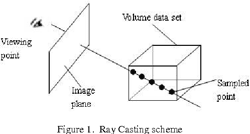
\includegraphics[width=.8\linewidth,natwidth=250,natheight=134]{RayCasting1.png}
  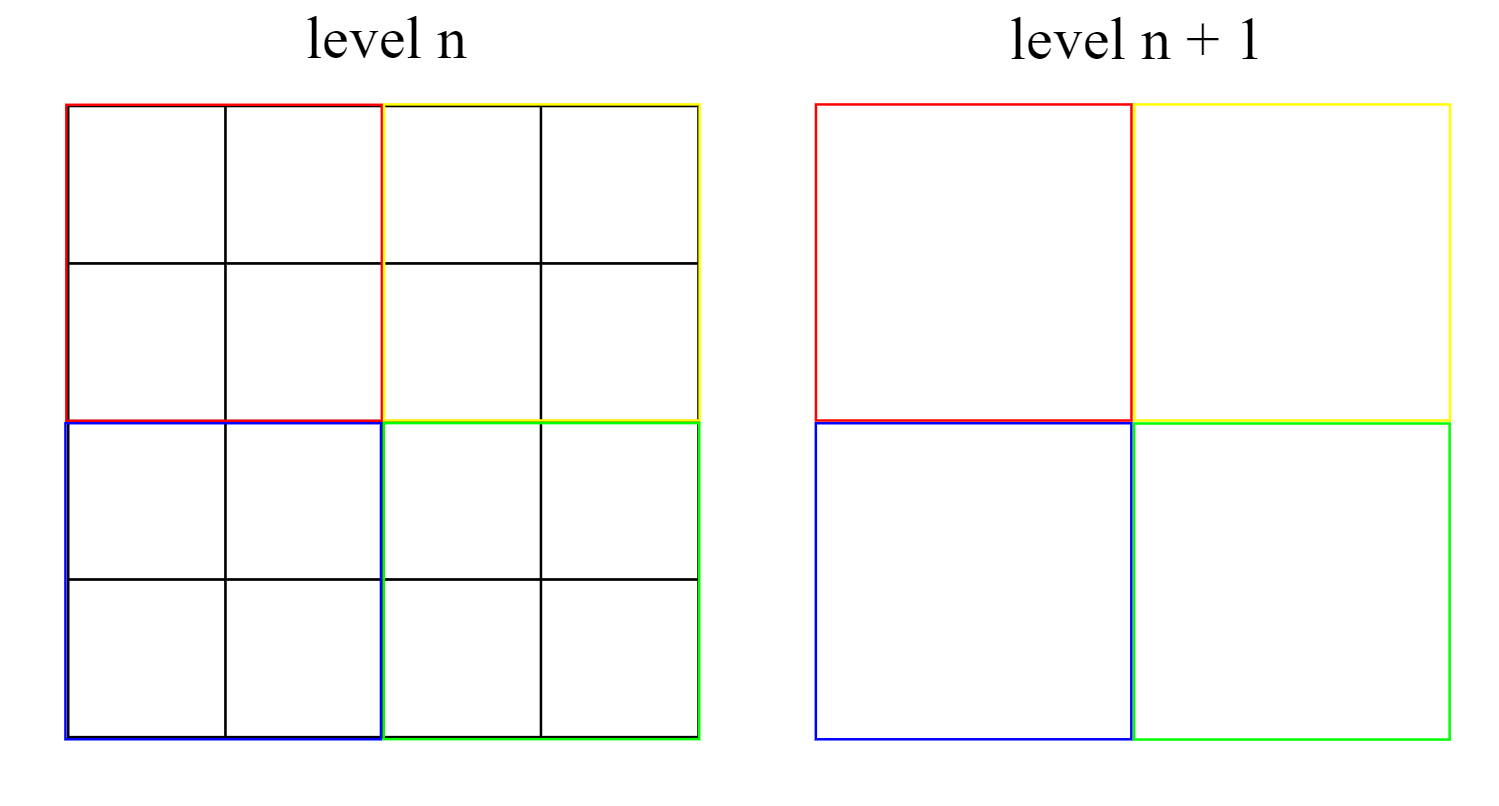
\includegraphics[width=.8\linewidth]{pyramide.png}
  \parbox[t]{.9\columnwidth}{\relax}
  %
  \caption{\label{fig:firstExample}
         Simplified 2 dimensional example of 2 levels of a pyramid. Each pixel in level n +1 contains 4 pixel of the lower level. In 3 dimensions, 8 voxels of the lower level are contained in one voxel of the upper level.}
\end{figure}


\subsection{Fixed Step Multiresolution}
This optimization makes use of the above described average pyramid, and works by casting the rays through a level of the pyramid, instead of the original data. As previously mentioned, when casting a ray trhough level $n$, the distance between the sampling points is $2^n$ times larger than the normal distance. The level through which the rays are cast can be freely choosen. Similar to mip-maps, it is also possible to select a real number as a level, in this case, the levels above and below the chosen level are rendered, and the two results are interpolated together. Since this would require rendering the pyramid at two levels, this is slower than just choosing a natural number as a level and recommendable only if a smooth transition between two levels is needed, like in gaze directed rendering as desribed by Levoy(CITE!!). The higher the level the faster the algorithms works, but the lower the resolution becomes.

\subsection{Presence Acceleration}
This algorithm uses an average and a maximum pyramid. The maximum pyramid is used to quickly find regions with low opacity, where the average pyramid is used to sample at a lower resolution. The idea behind this algorithm is that low opacity regions do not contribute much to the final result, and can be therefore be sampled more sparsely.
The algorithm works by casting each ray through the maximum pyramid at the highest level. For each cell that is intersected, it checks if the opacity value of that cell is larger than some user provided treshold $k \in [0, 1]$.
If so, that means that the average opacity in that region is not small enough, and we move down one level in the pyramid in the hope of finding such a region at a lower resolution.
However, if the opacity is smaller the average pyramid is used to approximate that cell. [MORE DETAILS?]
Once a cell in the maximum pyramid has been checked, the algorithm advances to the next cell and checks if the new cell has the same parent as the old one. If not, we move up one level in the pyramid. This is done to ensure that the algorithm always advances with the largest possible step size.
After that, the same procedure is repeated until the ray has moved through the entire pyramid.
Further improvements to this algorithm can be madeby considering two observations:
Firstly, it is very rare for the cell in the highest level of the maximum pyramid to have a $\alpha$ lower than $k$ (this would mean that the entire volume is almost completly transparent). It is therefore preferable not to start at the highest level but samewhat lower. XXX suggests in [CITE] to start two levels lower.
Secondly, finding the cells that the ray intersects is a computationally relatively expensive operation that might not amortize itself at lower levels. Therefore, it might be more effiecient to start sampling at the lowest level of the average pyramid before the lowest level of the maximum pyramid is reached. XXX suggests in [] to sample level 0  of the average pyramid once level 2 of the maximum pyramid is reached. [REFORMULATE?]



\subsection{Homogenity Acceleration}
This algorithm works conceptually the same as presence acceleration. The difference is that homogenity acceleration takes fewer samples in regions with high homogenity and not in regions of low opacity. The idea behind the algorithm is that in a region where all voxels are very similar to each other, accumulating x different samples and accumulating the average of the region x times yields a very similar result. The algorithm works in the same way as presence acceleration, only the maximum pyramid is replaced with the range pyramid.
\subsection{$\beta$  Acceleration}
%-------------------------------------------------------------------------






\bibliographystyle{eg-alpha-doi}
\bibliography{bib}



%-------------------------------------------------------------------------
% bibtex
%\bibliographystyle{eg-alpha-doi} 
%\bibliography{bib}       

% biblatex with biber
%\printbibliography                

%-------------------------------------------------------------------------


